\documentclass[12pt]{article}
\usepackage{amsmath,amssymb,amsthm,enumerate,dsfont}
\usepackage{pdfpages}
\usepackage[a4paper,bindingoffset=0.2in,%
left=0.8in,right=0.8in,top=1in,bottom=1in,%
footskip=.25in]{geometry}

\newcommand{\prob}[1]{\textbf{P}(#1)}

\title{Statistical Theory Homework 3}
\date{\today}
\author{Bohao Tang}

\begin{document}
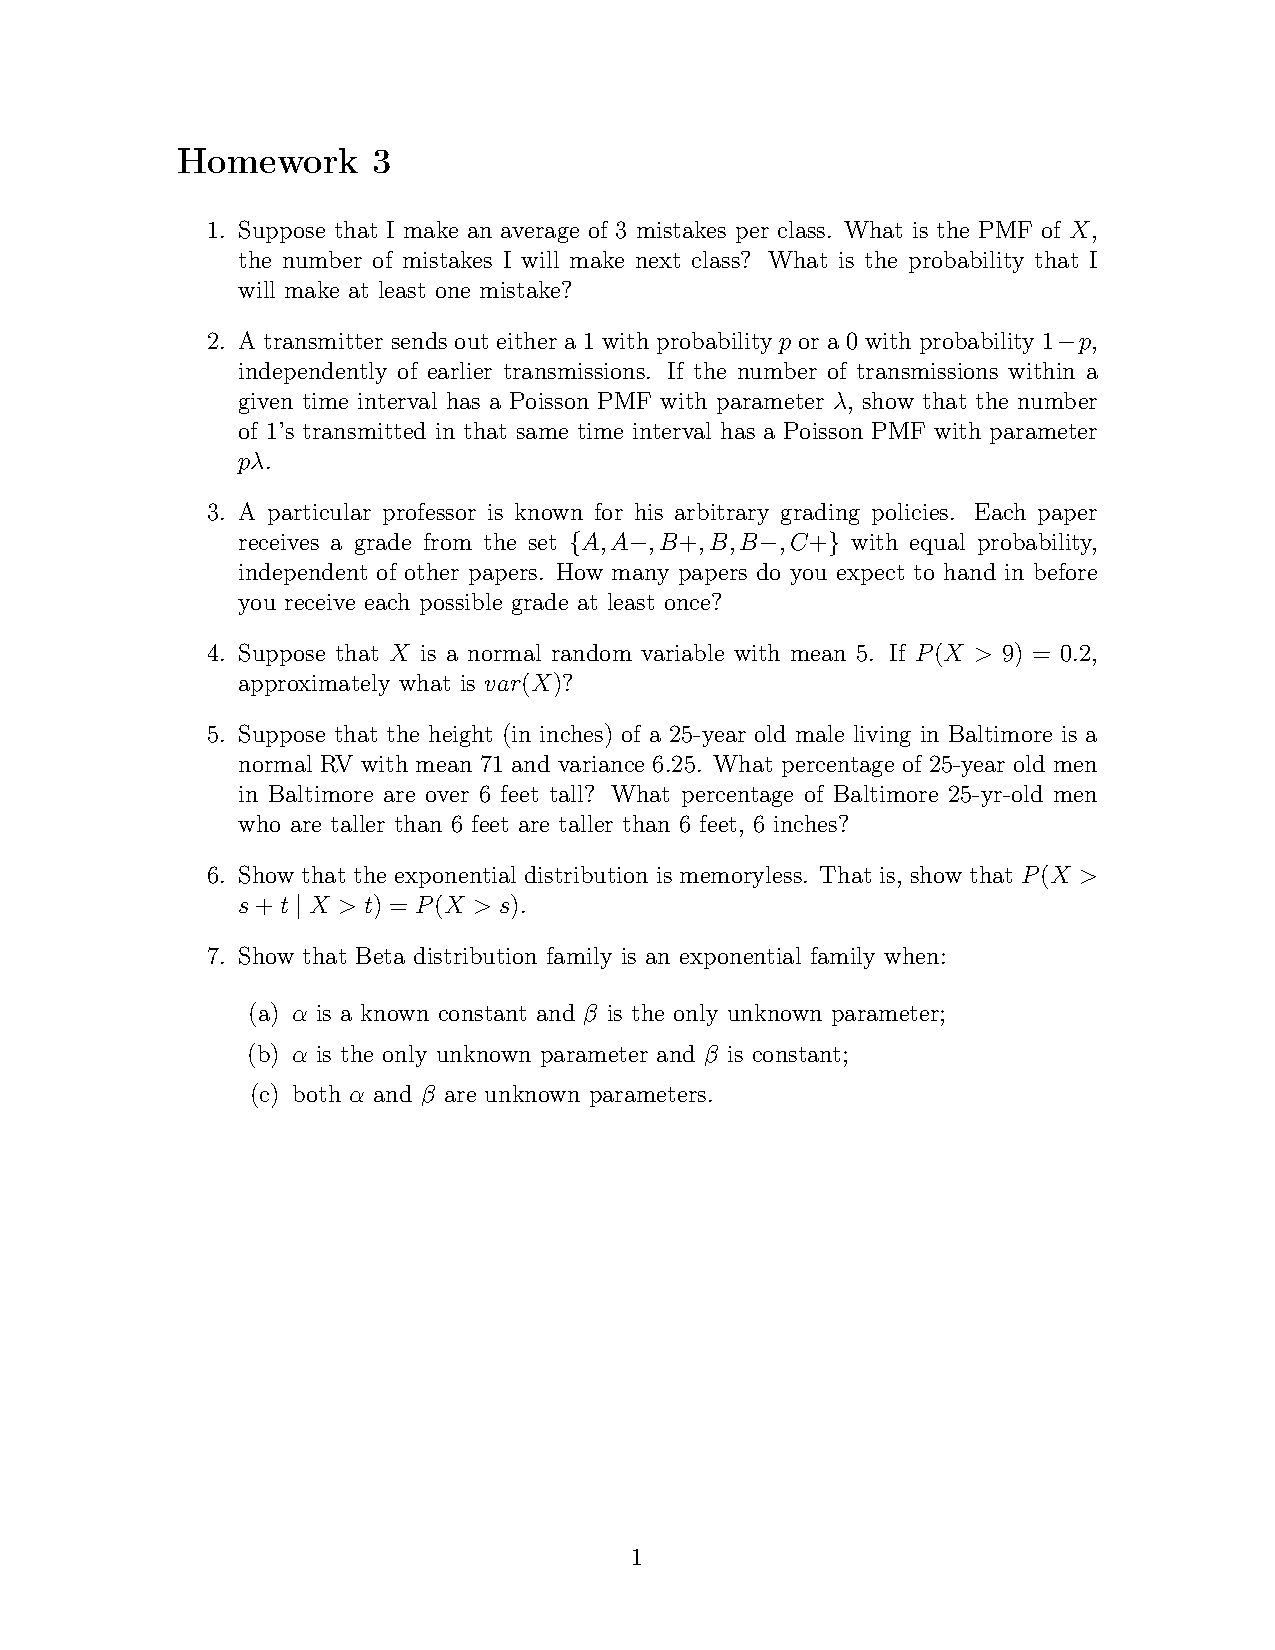
\includepdf[pages=-]{HW_3.pdf}
\maketitle

\begin{enumerate}
    \item
    It's reasonable to suppose that the number of mistakes you make in each class $X$ is independent and follow a Poisson distribution
    $Poi(\lambda)$, then from the question we get that $\lambda = \mathbb{E}[X] = 3$. Therefore the PMF of $X$ is:
    $$\textbf{P}(X = n) = \frac{3^n}{n !} e^{-3}$$
    where $n \in \mathbb{N}$ ($0 \in \mathbb{N}$). And we have:
    $$\textbf{P}(X \ge 1) = 1 - \textbf{P}(X = 0) = 1 - e^{-3}$$
    \item
    Denote $X$ to be the number of transmissions in this interval and $Y$ be the number of 1's transmitted.
    Then we have:
    \begin{eqnarray}
        \prob{Y = k} &=& \sum_{n=0}^{\infty} \prob{Y = k; X = n} = \sum_{n=0}^{\infty} \prob{Y = k | X = n} \prob{X = n} \\
                     &=& \sum_{n=k}^{\infty} \prob{Y = k | X = n} \prob{X = n} = \sum_{n=k}^{\infty} \binom{n}{k} p^k (1-p)^{n-k} \frac{\lambda^n}{n !} e^{-\lambda} \\
                     &=& \frac{e^{-\lambda} p^k \lambda^k}{k !} \sum_{n=k}^{\infty}\frac{[(1-p)\lambda]^{n-k}}{(n-k)!} = \frac{e^{-\lambda} p^k \lambda^k}{k !} \cdot e^{\lambda - p\lambda} \\
                     &=& \frac{(p\lambda)^k}{k !} e^{-p\lambda}
    \end{eqnarray}
    Therefore Y $\sim Poi(p\lambda)$.
    \item
    Let $X$ be the number of papers you hand in before you receive each possible grade at least once. 
    Actually I think there are two interpretation of the word "before". One is that you hand in your $X^{th}$ paper, and after grading, you firstly get every grade.
    And the other is that right after you send your $X^{th}$ paper (that is when you send your $(X+1)^{th}$ paper), you firstly get every grade.
    
    In this solution, I think the first interpretation is more meaningfull, although they are nearly the same (if you use the second interpretation, plus my answer with $1$).

    We then easy to see that $X = X_1 + X_2 + X_3 + X_4 + X_5 + X_6$, where $X_i$ is the paper you need to get a new type grade after you already get $i - 1$ types of grades.
    Also, $X_i$ will follow a geometric distribution with success probability $\frac{6-i+1}{6}$. Because every grading of paper is independent, to get a new type of grade, you are just repeat doing iid experiments until success.
    
    Therefore we have $\mathbb{E}[X] = \sum_{i=1}^{6} \mathbb{E}[X_i] = \sum_{i=1}^{6} \frac{6}{7-i} = \frac{147}{10}$.
    \item
    Suppose $var(X) = \sigma^2$, then $(X - 5) / \sigma$ follows the standard normal distribution. Then $\prob{X > 9} = 0.2 \Rightarrow \prob{\frac{X-5}{\sigma} > \frac{4}{\sigma}} = 0.2$, 
    call R function "qnorm(0.8)", we can get that $\frac{4}{\sigma} = 0.8416212$. Therefore $var(X) = 22.58846$.
    \item
    We use R function "pnorm" to do the calculation. Here suppose $H$ be the random variable of height:
    \begin{eqnarray}
        \prob{H > 6'} &=& 1 - \prob{H \le 72"} \\
                            &=& 1 - \prob{\frac{H-71}{\sqrt{6.25}} \le \frac{72-71}{\sqrt{6.25}}} \\
                           &=& 1 - \text{pnorm}(\frac{72-71}{\sqrt{6.25}})\\
                            &=& 0.3445783\dots \doteq 34.458\% \\
        \prob{H > 6'6" | H > 6'} &=& \frac{\prob{H > 78 ; H > 72}}{\prob{H > 72}} \\
                           &=& \frac{1 - \text{pnorm}(\frac{78-71}{\sqrt{6.25}})}{1 - \text{pnorm}(\frac{72-71}{\sqrt{6.25}})} = 0.00741525\dots \\
                          &=& 0.7415\% 
    \end{eqnarray}
    \item
    Suppose $X$ follows exponential distribution $exp(\lambda)$, then we have $\prob{X > s} = e^{- \lambda s}$, for all $s \ge 0$.
    Therefore:
    \begin{eqnarray}
        \prob{X > s + t | X > t} &=& \frac{\prob{X>s+t;X>t}}{\prob{X>t}} = \frac{\prob{X>s+t}}{\prob{X>t}} \\ 
                                 &=& \frac{e^{-s-t}}{e^{-t}} = e^{-s} = \prob{X > s} 
    \end{eqnarray}
    \item
    Suppose $X$ follows a Beta distribution $Be(\alpha,\beta)$. Then its pdf is: 
    $$f(x;\alpha,\beta) = \frac{x^{\alpha-1}(1-x)^{\beta-1}}{B(\alpha,\beta)}$$
    \begin{enumerate}[(a)]
        \item
        Given $\alpha$ a known constant, we have:
        $$f(x;\beta) = \frac{1}{B(\alpha,\beta)} \cdot x^{\alpha -1} \mathds{1}_{0\le x \le1} \cdot exp\{(\beta-1)\ln(1-x)\}$$
        Therefore it is of exponential family with $h(\theta)=\frac{1}{B(\alpha,\beta)};\ c(x)=x^{\alpha -1} \mathds{1}_{0\le x \le1};\ \omega(\theta)=(\beta-1);\ t(x)=\ln(1-x)$.
        \item
        Given $\beta$ a known constant, we have:
        $$f(x;\alpha) = \frac{1}{B(\alpha,\beta)} \cdot (1-x)^{\beta -1} \mathds{1}_{0\le x \le1} \cdot exp\{(\alpha-1)\ln(x)\}$$
        Therefore it is of exponential family with $h(\theta)=\frac{1}{B(\alpha,\beta)};\ c(x)=(1-x)^{\beta -1} \mathds{1}_{0\le x \le1};\ \omega(\theta)=(\alpha-1);\ t(x)=\ln(x)$.
        \item
        In general, we have:
        $$f(x;\alpha,\beta) = \frac{1}{B(\alpha,\beta)} \cdot \mathds{1}_{0\le x \le1} \cdot exp\{(\alpha-1)\ln(x) + (\beta-1)\ln(1-x)\}$$
        Therefore it is of exponential family with $h(\theta)=\frac{1}{B(\alpha,\beta)};\ c(x)=\mathds{1}_{0\le x \le1};\ \omega_1(\theta)=(\alpha-1);\ \omega_2(\theta)=(\beta-1);\ t_1(x)=\ln(x);\ t_2(x)=\ln(1-x)$.
    \end{enumerate}
\end{enumerate}

\end{document}